\documentclass[a4paper]{report}
%\usepackage{fullpage}
\usepackage{listings}
\usepackage{caption}
\usepackage{url}
\usepackage{tikz}
%\usepackage{courier}

\begin{document}

\lstset{ %
language=Haskell,               % the language of the code
basicstyle=\ttfamily,       % the size of the fonts that are used for the code
numberstyle=\footnotesize,      % the size of the fonts that are used for the line-numbers
stepnumber=2,                   % the step between two line-numbers. If it's 1, each line 
% will be numbered
numbersep=5pt,                  % how far the line-numbers are from the code
showspaces=false,               % show spaces adding particular underscores
showstringspaces=false,         % underline spaces within strings
showtabs=false,                 % show tabs within strings adding particular underscores
tabsize=2,                      % sets default tabsize to 2 spaces
captionpos=b,                   % sets the caption-position to bottom
breaklines=true,                % sets automatic line breaking
xleftmargin=30pt,
breakatwhitespace=false,        % sets if automatic breaks should only happen at whitespace
title=\lstname,                 % show the filename of files included with \lstinputlisting;
escapeinside={\%*}{*)},         % if you want to add a comment within your code
morekeywords={*,...}            % if you want to add more keywords to the set
}


\title{Lazy functional programming language targeting Low Level Virtual Machine}
\author{\textit{Author:}\\Piotr Micha\l{} Kaleta\\\\\emph{Supervisor:}\\dr W\l{}odzimierz Moczurad}
\date{\today}

\maketitle
\pagenumbering{roman}

\newpage
\thispagestyle{empty}
\mbox{}

\Huge
\begin{abstract}
  \normalsize
  \center
  This paper describes the design and Haskell implementation of a lazy
  programming language called Kivi. It is higly influenced on both Haskell's
  syntax as well as the way that computations are performed. However it generates
  the \textit{Low Level Virtual Machine}\cite{website:llvm} Intermediate
  Representation code as the output, which is then assembled and compiled to
  native code by LLVM.
\end{abstract}


\renewcommand{\abstractname}{Acknowledgements}
\begin{abstract}
  \normalsize
  \center
  TODO: napisac
  \begin{flushright}
    Piotr Kaleta
  \end{flushright}
\end{abstract}

\normalsize
\pagenumbering{arabic}

\tableofcontents

\chapter{Introduction}

This paper describes the design and implementation of a lazy functional
language compiler. The implementation is based on the
\textit{G-machine}\cite{jones87} and uses \textit{lazy graph reduction} to
perform evaluation.

The compilation process is implemented as a set of passes that eventually
transforms the source code into simple intermediate language \textit{lambda
calculus} enriched with let(rec) expressions. It would be possible to implement
compiler using less passes than I did, or maybe even one, but such clear
separation made things simpler to both develop and debug as well. Besides now
the compiler is very modular and inserting additional passes could be done with
no harm, which wouldn't be that easy if I'd used one pass only instead.


In following chapters I am going to describe the process of translating
\textit{Lambda Calculus} into \textit{G-code} instructions.  Finally these
instructions will either be evaluated by the interpreter or compiled down to
LLVM intermediate representation and further to native code by LLVM
infrastructure compilers. Design and implementation of both of these concepts
will be described in separate chapters.

TODO: Opis po kolei czesci dokumentu

\section{Implementation language - Haskell}


\chapter{Parsing}

In order to translate the source of \textit{Kivi} into \textit{Lambda Calculus}
it has to be available in a structured form so thate later passes could easily
traverse it. \textit{Abstract Syntax Trees}\cite{wiki:ast} has been widely adopted as a
standard form of keeping the representation of source code in memory. The
process of reading the input source file and producing AST from it is called
\textit{parsing}.
I've chosen to implement a simple parser, in a similar manner as in
\cite{joneslester00} as it seemed as the simplest approach to me then. Now, as
the parser has grown, I'd strongly consider rewriting it to use parser combinator
library such as \cite{website:parsec} instead.  The parsing consists of two
passes. As previously mentioned such separation makes implementation and
reading the code easier. Thus parsing consist of:

\begin{itemize}
  \item Firstly \textit{lexical analysis} implemented by \texttt{lex} in
    \texttt{Lexer.hs} module extracts \textit{tokens} from plain text.
    \textit{Tokenization} is the process of demarcating and possibly
    classifying sections of a string of input characters. The resulting tokens
    are then passed on to further processing.
  \item \textit{Syntax analysis} is the process of analyzing the stream of
    tokens and building an \textit{Abstract Syntax Tree} from it.
\end{itemize}

TODO: Grammar of the language

This two-phase process is implemented as\footnote{Where \texttt{PatProgram}
is program containing patterns}:
\begin{verbatim}
  parse :: String -> PatProgram
  parse = syntax . lex
\end{verbatim}

\section{Lexical analysis}

The types for lexer are following:
\begin{verbatim}
  type Token = String
  type TokenInfo = (Int, Token)
\end{verbatim}
Where \texttt{TokenInfo} consist of line number and a token string itself.

The heart of \textit{lexical analyser} is the \texttt{lex'} function. It works
by classifying the parts of remaining input based on first characters.
Building number tokens may be a nice example of how it works:

\begin{lstlisting}[label=lex_comment,caption={Building tokens from numbers.}]
lex' (c : cs) lnum | isDigit c =
    (lnum, numToken) : lex' restCs lnum
        where
        numToken = c : takeWhile isDigit cs
        restCs = dropWhile isDigit cs
\end{lstlisting}


\section{Syntax analysis}
qwfofqw
efeqw
f
TODO: jak powstaje drzewo ast przedstawic tutaj datatype ktory sluzy do
trzymania ast


\chapter{Translation to Lambda Calculus}

In this chapter I'm going to present the process of transformation of a
high-level functional language into a simple intermediate form - \textit{lambda
calculus}. In the first part I'll show \textit{Kivi}'s syntax, its
constructs and structures. Later on the desired output form -
\textit{Lambda Calculus} will be shown. The rest of the chapter will
consist of ways to translate the first form into another.

\section{Syntax}
Source of \textit{Kivi}'s program consist of set of
\textit{supercombinators}\cite{wiki:supercombinator}. Supercombinator is an
expression consisting of either constants or other supercombinators and
doesn't contain any free variables in its body. Supercombinators might have
arguments, and those which doesn't are called \textit{constant applicative forms}
(or CAFs for short). Listing~\ref{supercombinator_ex} shows the simple
supercombinator with one argument.

\begin{lstlisting}[label=supercombinator_ex,caption={Simple supercombinator.}]
  sqr x = x * x
\end{lstlisting}

There is one special supercombinator called \textit{main}, that takes no
arguments. It is the entry point for program execution. If there's no
\textit{main} CAF present in Kivi's source, both compiler and interpreter
should issue specific error message.

\subsection{Case expressions}
The purpose of case expression is to allow the programmer to control the flow
of program execution via a multiway branch. The semantics of case is rather
simple. First, the expression under case is evaluated and then based on result,
the appriopriate execution path is chosen. Example of case expression is
presented in Listing~\ref{lst:case_ex}.

\begin{lstlisting}[label=lst:case_ex,caption={Fibonacci with case}]
  fib n =
      case n of
          0 -> 1;
          1 -> 1;
              n -> fib (n-1) + fib (n-2);

  main = fib 10
\end{lstlisting}

% TODO: zmienic \ref{xxx} na \ref{lst:xxx}
\subsection{Local bindings}
Supercombinators provides the ability to define local definitions using
\texttt{let} keyword. The scope of variables defined using \texttt{let} is
enclosed by the expression following \texttt{in} keyword. The example use of
local binding is presented in Listing~\ref{let_ex}


\begin{lstlisting}[label=let_ex,caption={Local \texttt{let} binding.}]
  sum x y = x + y;

  main =
      let x = 1
          y = 2
      in
          sum x y
\end{lstlisting}

\subsection{Recursive local bindings}
In order to define mutually recursive bindings using \texttt{let} one has to use the
special \texttt{letrec} construct as shown in Listing~\ref{factorial_letrec_ex}


\begin{lstlisting}[label=factorial_letrec_ex,caption={Factorial function using \texttt{letrec}.}]
  sum x y = x + y;

  main =
      letrec fac n =
          case n == 0 of
              True -> 1;
              False -> n * fac (n-1)
      in
          fac 5
\end{lstlisting}

\subsection{Where clauses}
Another way of creating recursive definitions is using the \texttt{where}
clause. Internally it will be translated into letrec binding. Example use of
\texttt{where} clause is shown in Listing~\ref{factorial_where_ex}

\begin{lstlisting}[label=factorial_where_ex,caption={Factorial function using \texttt{where}.}]
  main = fac 5
      where
          fac n = case n == 0 of
              True -> 1;
              False -> n * fac (n - 1)
\end{lstlisting}

\subsection{Lambda abstractions}
Functions in Kivi can be defined in two ways. The first one is the top level
supercombinators that has already been discussed. The other option is to define
them as \textit{lambda abstractions}. This concept is similar to \textit{anonymous
functions} used in imperative languages. The syntax for defining lambda
abstractions is presented in Listing~\ref{lambda_ex}.

\begin{lstlisting}[label=lambda_ex,caption={Lambda abstraction}]
  f = (\x . x * 2) 42
\end{lstlisting}

In this example the lambda abstraction which doubles the arguments value is
created and then applied to 42 yielding 84 as result.

During compilation process programs containing lambda abstractions are
transformed into their equivalents with lambda abstractions substituted for top
level supercombinators. This process is called \textit{lambda lifting} and is
described in more detail in chapter~\ref{lambda_lifting}.

\subsection{Pattern matching}

Pattern matching consists of specifying patterns to which some data should
conform and then checking to see if it does, as well as deconstructing the data
according to those patterns. So in other words, using pattern matching you can
recognize values, bind variables to those values and break structures down into
parts.
Patterns are matched in order they are defined in source code. Once a
successful branch is found, the right-hand-side expression is evaluated and
result returned. None of the following patterns is checked. If after checking
all patterns it turns out that none of them matches the argument, the error is
returned.

\begin{lstlisting}[label=pattern_matching_ex,caption={Factorial using pattern matching.}]
  fac 0 = 1
  fac n = n * fac (n - 1)
\end{lstlisting}

In Listing~\ref{pattern_matching_ex} a recursive supercombinator \texttt{fac}
calculating factorial is defined. There are two cases\footnote{To be honest
there are three cases, but for simplicity reasons we assume that
\texttt{fac} is called only for non-negative integers}. Either the
argument is 0 and then the result is 1, or argument is other than than 0 and
then we progress recursively. The factorial definition is expressed very
clearly by means of pattern matching.
Pattern matching is also very useful when it comes to dealing with data
types as we'll see in next section.

\subsection{Structured Data Types}
Data types in Kivi are defined using \texttt{data} keyword, giving the name of
new type as well as its constructors and arities. Together with pattern matching they
provide a very powerful mechanism for dealing with structured entities.

\begin{lstlisting}[label=data_type_ex,caption={Calculating length of list.}]
  data List = Nil 0 | Cons 2;

  length Nil = 0;
  length (Cons x xs) = 1 + length xs
\end{lstlisting}

In Listing~\ref{data_type_ex} a data type \texttt{List} is declared as well as
supercombinator calculating the length of a list by means of pattern matching.
In first case argument is pattern matched to the \texttt{Nil} constructor. If
matching succeeds it means that the list is empty, therefore its length is 0.
In next case the argument is matched to second \texttt{List} constructor, that
is \texttt{Cons}. If argument matches, the \textit{tail} of the list is bound to
\texttt{xs} variable and right hand side of that branch is evaluated.

\subsection{Function application and Currying}
% TODO: write
\section{Lambda Calculus}

\section{Translation to Lambda Calculus}
The process of translating a high-level functional language to \textit{lambda
calculus} might be considered as a set of program transformations. Each such
transformation is meant to simplify \footnote{or help with further
transformations} the program given as its input, eventually leading to the
expected \textit{enriched lambda calculus} form.
All those transformations accept some form of the program as input and yield
the simplified program as output. Therefore we might regard the compilation
process as a function composition of all transformations. This is exactly the
way the compilation is implemented in Kivi, and Haskell lets to express this
in a very concise way:

\begin{verbatim}
  run :: String -> String
  run = showResults
      . eval
      . compile
      . lambdaLift
      . lazyLambdaLift
      . analyseDeps
      . transformToLambdaCalculus
      . mergePatterns
      . tag
      . parse
\end{verbatim}

We have already discussed the parsing in previous chapters, so in the following
sections I'm going to provide a description of all remaining phases.

\subsection{Structured Data Types and Tagging}
In order to understand the need for this pass one has to know how structured
data types and their constructors are represented internally.
A custom data type declaration in Kivi might look like this one:

\begin{verbatim}
  data Tree = Leaf 1 | Branch 2
\end{verbatim}

This statement declares the new data type called \texttt{Tree} which can be
constructed in two ways. The common way of looking at the constructors is to
consider them as functions with zero or more arguments that return an instance
of a data type as a result. The \texttt{Tree} constructor is \texttt{Leaf} and
it has no further descendants. It takes one argument which is some kind of
value. The other way to construct a \texttt{Tree} is to create a \texttt{Branch}
taking two children (which also are \texttt{Tree}s) as arguments. For example,
conceptual representation of the following tree is shown in Figure~\ref{fig:tree}:

\begin{verbatim}
  Branch (Leaf 1) (Branch (Leaf 2) (Leaf 3))
\end{verbatim}

\begin{figure}[h!]
  \centering
    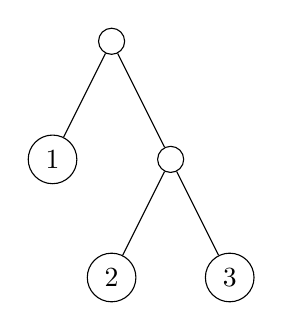
\begin{tikzpicture}
      \tikzstyle{every node}=[circle,draw]
      \node {}
          child { node {1} }
          child {
            node {}
              child { node {2} }
              child { node {3} }
          };
    \end{tikzpicture}
  \caption{Example of a tree.}
  \label{fig:tree}
\end{figure}

Constructors are used not only for object creation but also for decomposition
into parts as well as distinguishing the different types of trees based on
constructor. This feature is heavily used when pattern matching. For example
the code in Listing~\ref{lst:sqr_tree} uses it to create a new tree with values
that are square roots of values in original tree.

\begin{lstlisting}[label=lst:sqr_tree,caption={Creating a `square rooted` tree.}]
sqrTree (Leaf v) = Leaf (v * v)
sqrTree (Branch t1 t2) = Branch (sqrTree t1) (sqrTree t2)
\end{lstlisting}

\subsubsection{Built-in Data Types}
There are few types that are considered built-ins. These are lists, tuples,
and booleans. The ability to think of these common concepts in functional
programming as Structured Data Types makes the implementation straightforward
as I didn't have to treat these entities separately, instead I used a common
notion of data types.
\subsubsection{Booleans}
Boolean values in Kivi are implemented as a regular Structured Data Type having
two constructors representing true and false:

\begin{verbatim}
  data Boolean = True | False
\end{verbatim}

\subsubsection{Lists}
Lists are structures that allow storing a number of items. They
provide a set of operations on them that allowing to create other
lists\footnote{In Kivi lists as well as other types are immutable, which means
that you cannot modify its contents. Instead you create new values which may
differ from previous ones. }
Kivi provides a variety of way to define a list. First of all lists can be seen
as regular Data Type. Thus there are two constructors for a \texttt{List}
datatype. \texttt{Nil} and \texttt{Cons}:

\begin{verbatim}
  data List = Nil 0 | Cons 2
\end{verbatim}

\texttt{Nil} instantiates an empty \texttt{List} whereas \texttt{Cons} is meant
to \textit{construct} \texttt{List} given two elements: the \textit{head} and
\textit{tail}. List are recursive structures, thus \textit{tail} is another
list.

It turns out that creating a \texttt{List} is a task that occurs very often in
functional languages, therefore it would be nice not to have to write long
constructs such as this one to create 4-element \texttt{List}:

\begin{verbatim}
  Cons 1 (Cons 2 (Cons 3 (Cons 4 Nil)))
\end{verbatim}

Most functional languages allow programmer to express it in a much shorter way,
and Kivi does it too:

\begin{verbatim}
  [1,2,3,4]
\end{verbatim}

The same thing concern constructing lists given two elements. Kivi provides
`:`(colon) as construction operator for \texttt{List} type, so the programmer
would write:

\begin{verbatim}
  ((2+3) : [1,2,3,4])
\end{verbatim}
instead of:

\begin{verbatim}
  Cons (2+3)  [1,2,3,4]
\end{verbatim}

\subsubsection{Tuples}
Tuples are yet another way of storing multiple values in a single one. However
the difference between them and lists is significant. Tuples are
\textit{immutable} in a way that you cannot \textit{cons} to a tuple nor
decompose them into parts using pattern matching. Their main usage is when a
programmer knows in advance how many elements will he need to store.

There is a predefined number of tuple types that you can create, and currently
the bound is set to 4. This means that programmer is not allowed to create
tuples that contain more than 4 elements. This design decision is due to the
fact that from my perspective it's better to use custom Structured Data Type
for readability reasons. The limit of 4 however, is an experimental value and
might be changed.

This all means that tuples with different number of elements are different
types. Therefore there is no such thing as generic `Tuple` type. There are
however \texttt{Tuple0}, \texttt{Tuple1}, \ldots etc., representing tuples with
0 elements, 1 element, \ldots etc.

There are two ways to create a tuple either by using constructors or by a
special \textit{syntactic sugar} construct, similarly as in the case for lists.
These two ways for instantiating a 3-element tuple are equivalent, with the
preference for the second one, due to readability concerns:

\begin{verbatim}
  (((Tuple3 1) 2) 3)
\end{verbatim}
and
\begin{verbatim}
  (1, 2, 3)
\end{verbatim}

\subsubsection{Implementation and tagging}
Internally each data type consist of a list of constructors, each containing a
\textit{tag}, and \textit{arity}. Constructor tags should uniquely identify
each constructor therefore each tag should be different. The definitions
for \texttt{DataType} and \texttt{Constructor} type synonyms, as in
\textit{Common.hs} are as follows:

\begin{verbatim}
  type DataType = (Name, [Constructor])
  type Constructor = (Name, Int, Int)
\end{verbatim}

Because of the fact that there's no way to know in advance how many data type
declarations are there in source file I had to devise some way to assign a
unique tag for each of constructors that is not a built-in one. This is
precisely what the tagging phase is for. It works in two parts:

\begin{itemize}
  \item First it traverses the list of data types and its constructors in order
    to create a mapping between constructor name and its unique tag.
  \item Next the whole AST is recursively traversed and each
    \texttt{EConstrName} node is substituted for \texttt{EConstr} containing
    the previously associated tag and arity.
\end{itemize}

The definitions for those functionalities has been placed in
\textit{AbstractDataTypes.hs} file.


\subsection{Merging patterns}
\subsection{Transforming \texttt{let} expressions}
\subsection{Pattern Matching}
\subsection{Transforming \texttt{case} expressions}
\subsection{Dependency analysis}
\subsection{Lambda lifting}
\subsection{Lazy lambda lifting}



\chapter{G-Machine}
\section{Interpreter}
\section{LLVM Compiler}

\bibliographystyle{alpha}
\bibliography{kivi}

\end{document}
